\documentclass{beamer}

%Packages BEGIN
\usepackage{amsmath}
\usepackage{xeCJK} % use this package to set Chinese and English font separately
\usepackage{fontspec} 
 

%Packages END

%Style setting BEGIN
\usetheme{Madrid} 
\usecolortheme{default} 

% Serif font in Ubuntu. Choose the Chinese font available in your device
\setCJKmainfont{Noto Serif CJK TC}

% Serif font in Ubuntu. Choose the Chinese font available in your device
\setCJKmonofont{Noto Serif CJK TC}

% Serif font in Ubuntu. Choose the Chinese font available in your device
\setCJKsansfont{Noto Serif CJK TC}

\XeTeXlinebreaklocale "zh" % enabling auto linebreaks
\XeTeXlinebreakskip = 0pt plus 1pt % enabling auto linebreaks
 
%Style setting END

\title{Anki Auto-lookup}
\subtitle{A convenient tool for English learning}
\author[張家翔, 王昊謙, 徐鼎翔]
{B08901062 張家翔\inst{1} \and 
B07202020 王昊謙\inst{2} \and 
B07202037 徐鼎翔 \inst{2}}
 
\institute[NTU] % (optional)
{
	\inst{1}%
	Department of Electrical Engineering\\
	National Taiwan University
	\and
	\inst{2}%
	Department of Physics\\
	National Taiwan University
} 

\begin{document}

\frame{\titlepage} 

\begin{frame}
	\frametitle{Motivation}
	Anki: A cross-platform flashcard application, which supports images, HTML,
	\LaTeX, audio, etc.
	\begin{figure}[h]
		\centering
		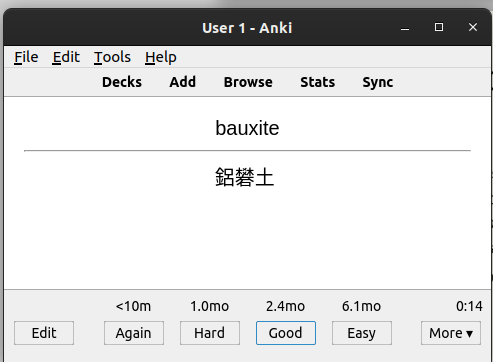
\includegraphics[width=0.55\linewidth]{./ankidesktop.png}
		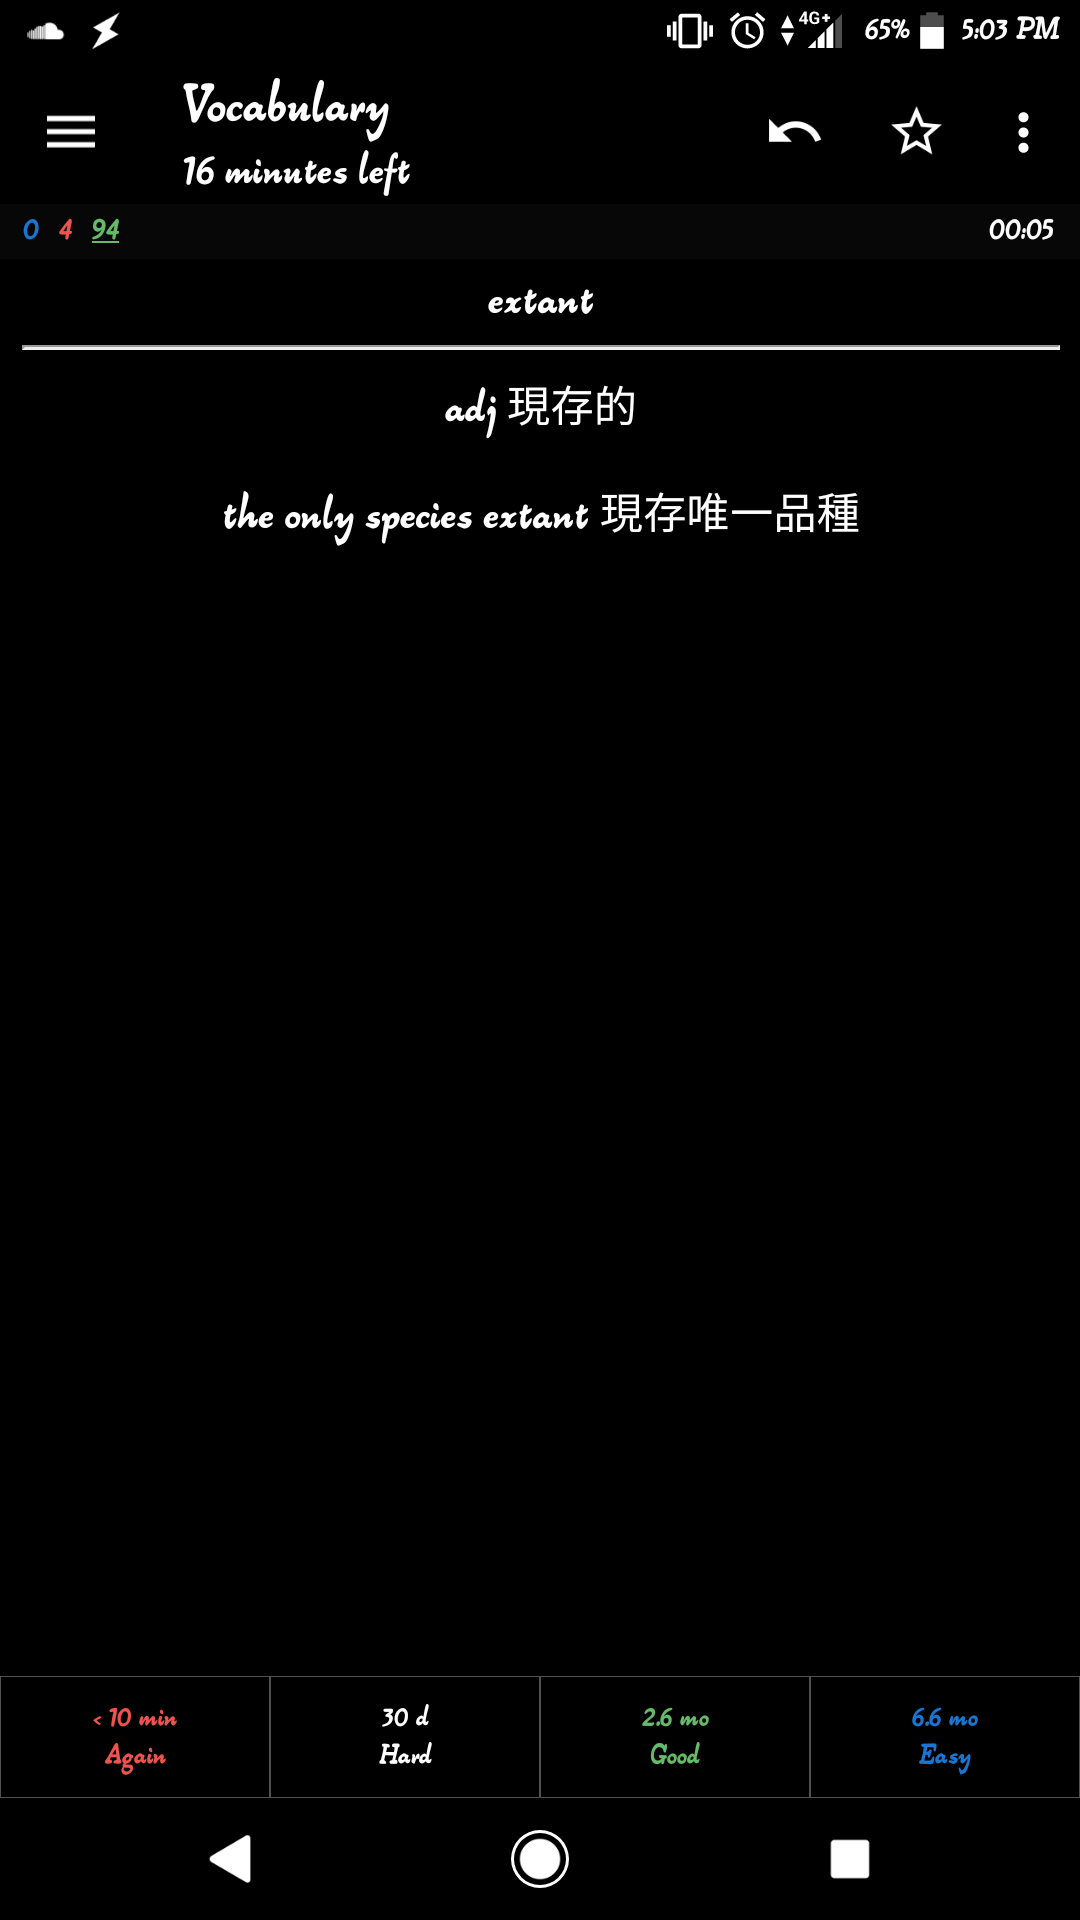
\includegraphics[width=0.28\linewidth]{./ankidroid.png}
		\caption{Anki on Ubuntu and Android.
		\label{fig:anki}}
	\end{figure}
\end{frame}

\begin{frame}{Motivation}
	\begin{enumerate}
		\item It is time-consuming to add new cards.
		\item More detailed definitions and example sentences are needed.
		\item Anki provides an API that can modify and add cards.
		\item Unknown words keep interrupting us while reading articles.
	\end{enumerate}
\end{frame}

\begin{frame}{Tasks}
	\begin{enumerate}
		\item A crawler to lookup definitions, pronunciation, and example
			sentences.
		\item Automatically add cards to our deck.
		\item Analyze an article, find difficult words and look them up.
		\item Find words in a picture (e.g. a picture of a page in a vocabulary
			book), then look them up.
	\end{enumerate}
	
\end{frame}


\end{document}
